\documentclass[11pt]{article}
\usepackage{ex-stile}
\usepackage{graphicx} 
\usepackage{rotating}

\begin{document}

\title{\textbf{Performance Evaluation Homework 4}}
\author{Ferhat Elmas}
\date{19.04.2012 Thursday}
\maketitle

\section*{Problem 1 - Running the Simulation}

I have run the simulation twice and I have uploaded generated log files to here[1] for one run.

\section*{Problem 2 - Power Exponent p}

     \begin{center}
     \begin{table}[ht]
     \centerline{
     \begin{tabular}{c}
	\begin{turn}{-90} \resizebox{4in}{!}{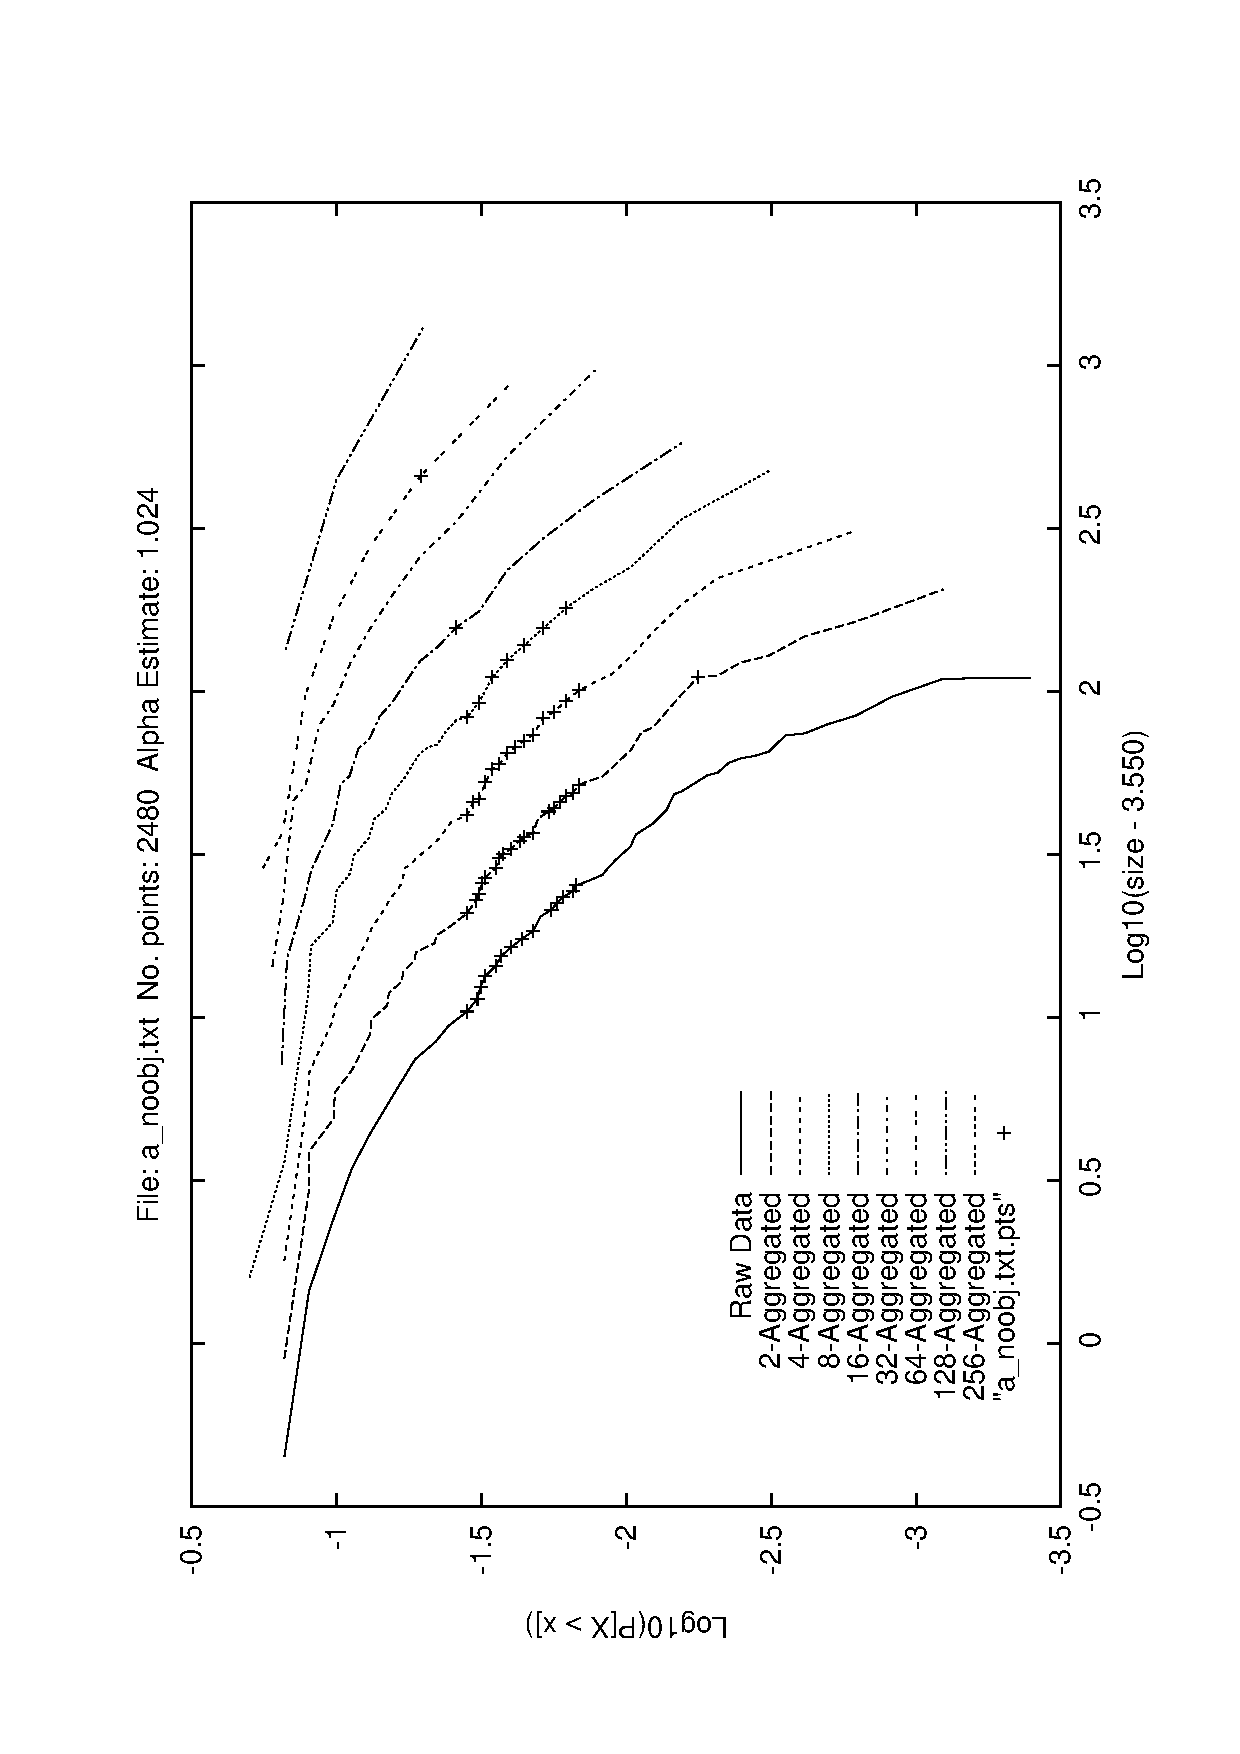
\includegraphics{p_noobj}} \end{turn} \\
     \end{tabular}} 
     \caption{Number of Embedded References}
     \label{q2:table1}
     \end{table}
     \end{center}

    \begin{center}
    \begin{table}[ht]
    \centerline{
    \begin{tabular}{c}
	\begin{turn}{-90} \resizebox{4in}{!}{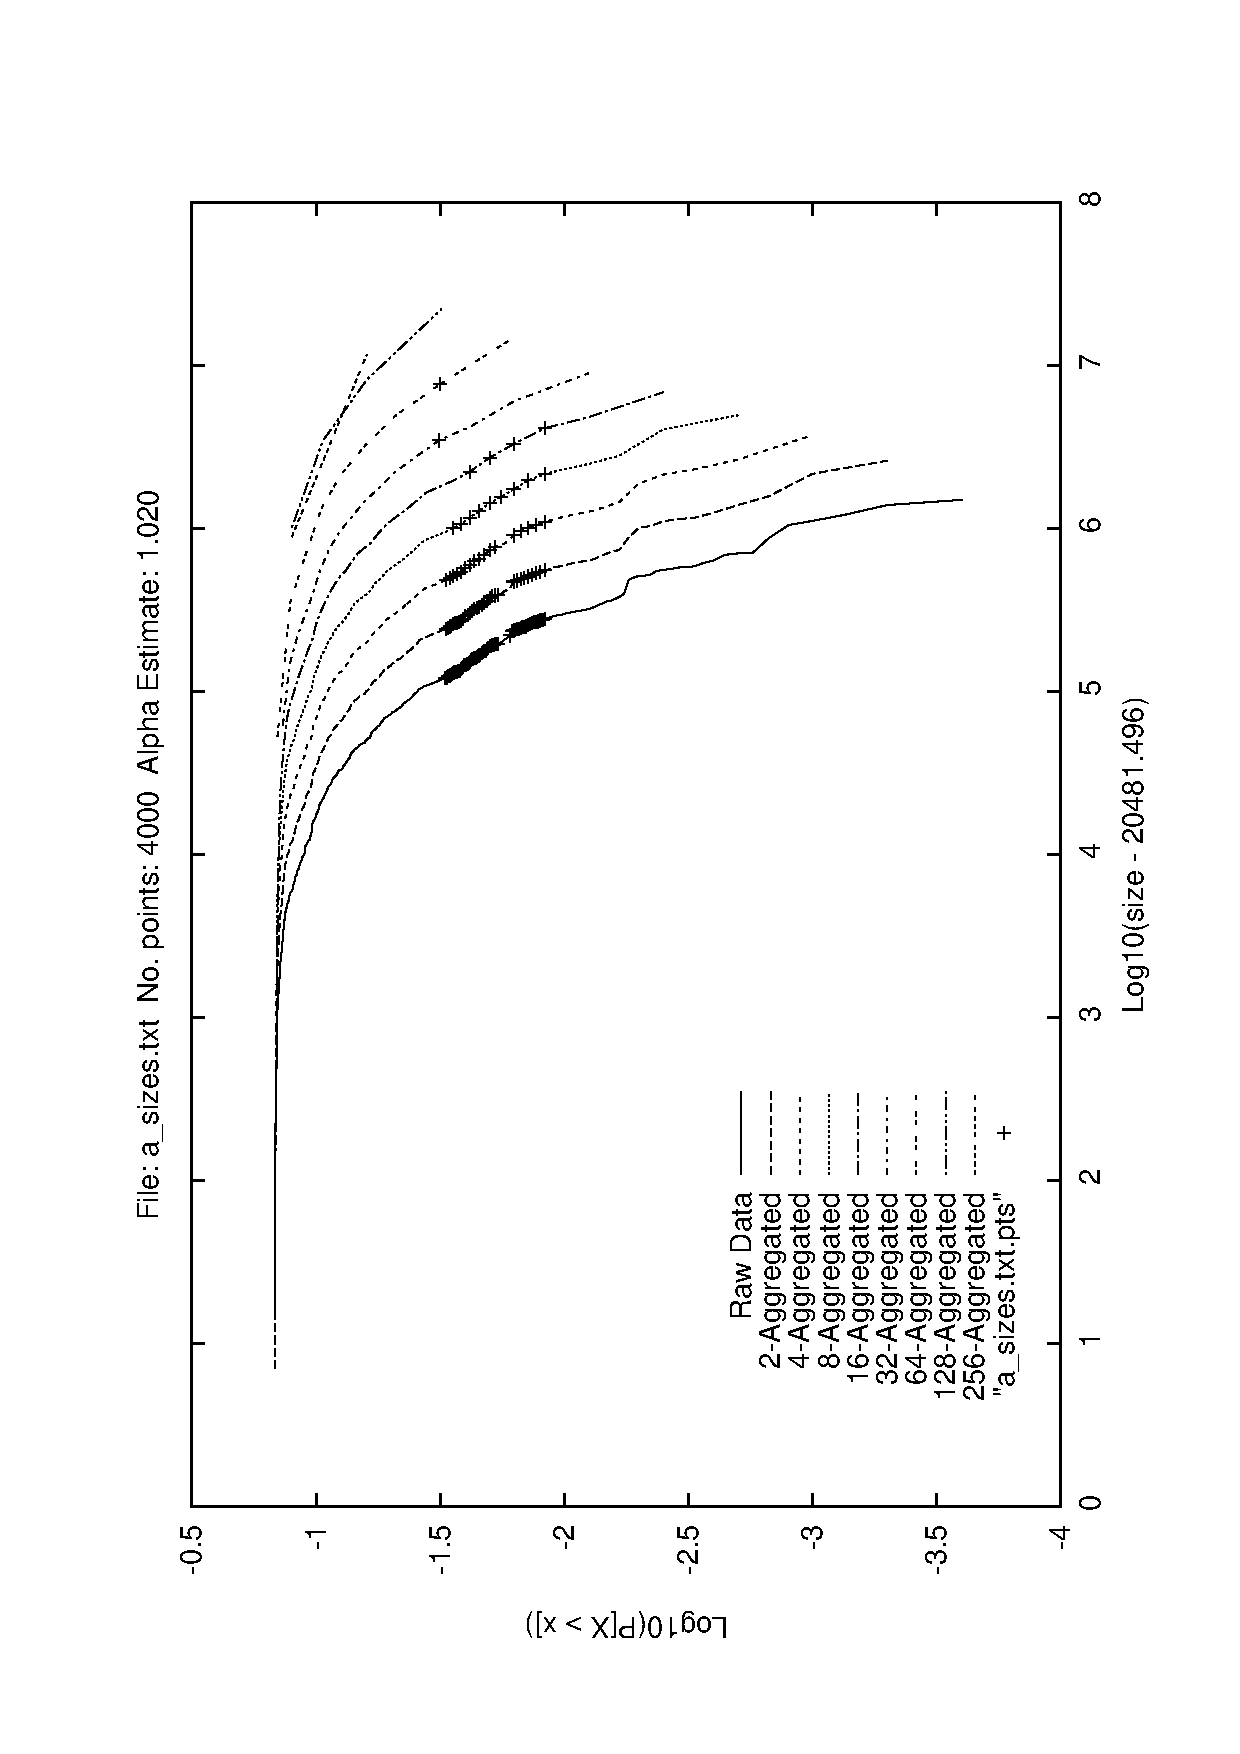
\includegraphics{p_sizes}} \end{turn} \\
     \end{tabular}} 
     \caption{File Sizes}
     \label{q2:table2}
     \end{table}
     \end{center}

     \begin{center}
     \begin{table}[ht]
     \centerline{
     \begin{tabular}{c}
	\begin{turn}{-90} \resizebox{4in}{!}{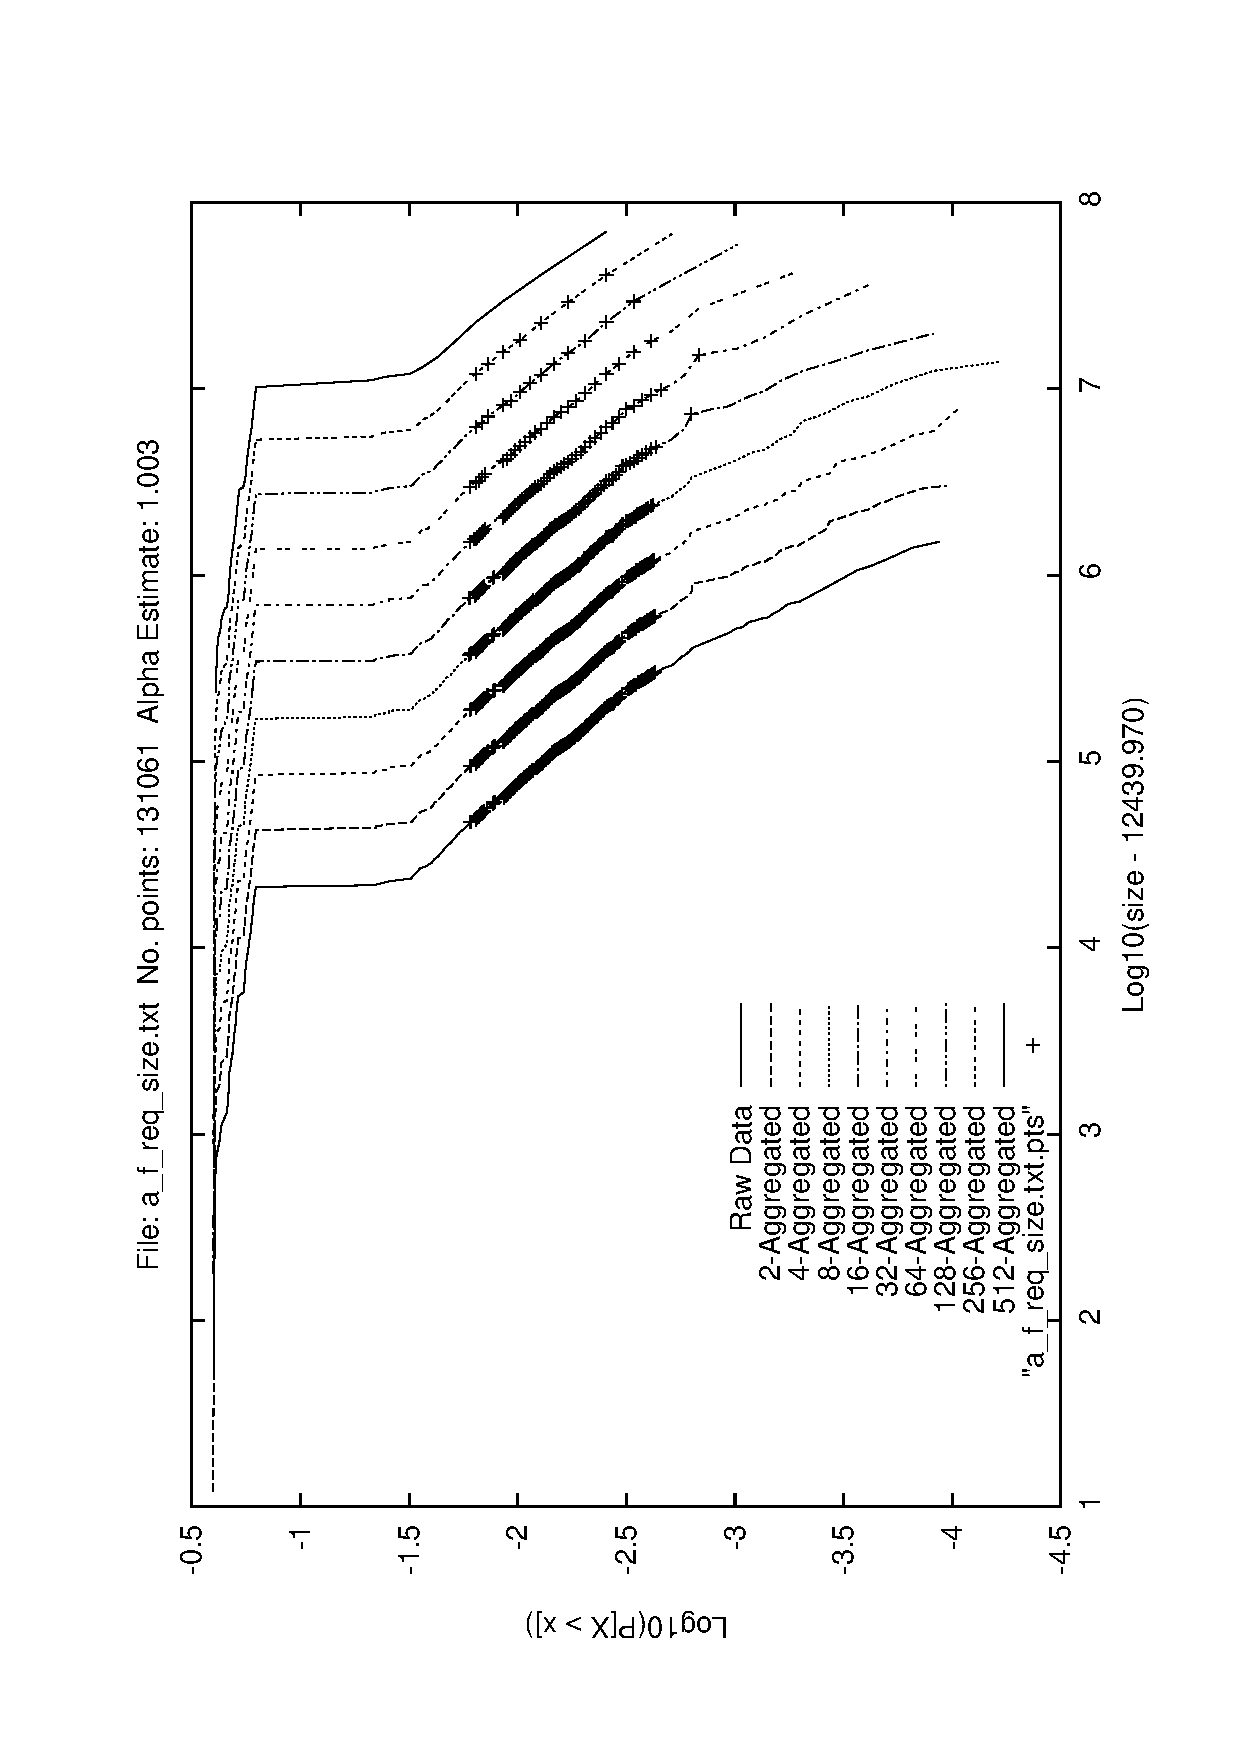
\includegraphics{p_f_req_size}} \end{turn} \\
     \end{tabular}} 
     \caption{File Request Sizes}
     \label{q3:table3}
     \end{table}
     \end{center}

\clearpage

\section*{Problem 3 - D and T values}

     \begin{center}
     \begin{table}[h]
     \centerline{
     \begin{tabular}{c}
	\resizebox{5in}{!}{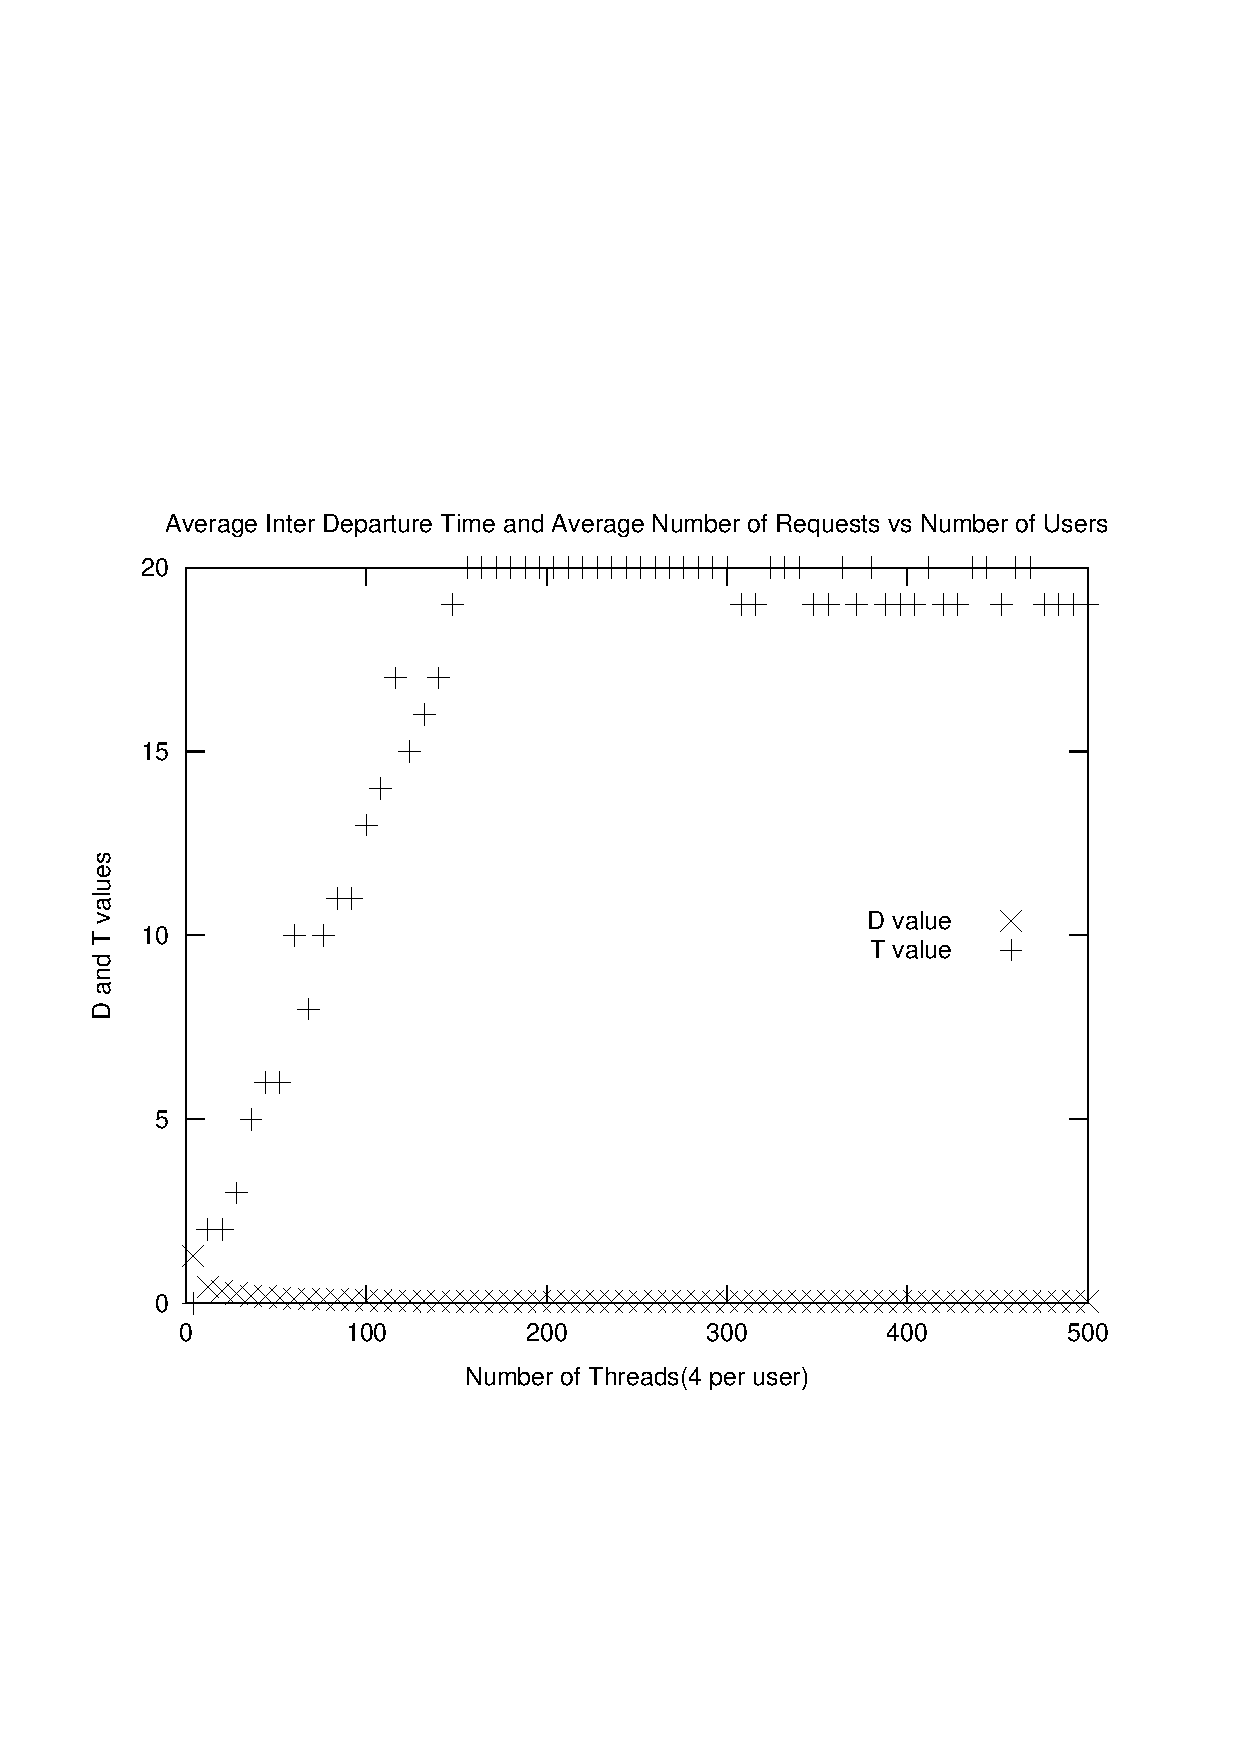
\includegraphics{dt}} \\
     \end{tabular}} 
     \caption{Average Inter Departure Time and Average Number of Serviced Request vs The number of the Users}
     \label{q3:table1}
     \end{table}
     \end{center}

When the number of the threads arrives at around 150, we see a saturation because when we continue increasing the number of the threads, the average number of the serviced request remains same at 19-20. Since we don't experience a decrease in the number of serviced requests, we can't say that there is a congestion collapse. However, there is a saturation for sure because we can't get more when we add more requests.

This is due to the client not the server, we use only one machine to stress the server but there is a limit on the Linux machine. At first, when we increase the number of the threads, client can do more frequent requests but after some time, it can't scale more because it needs context switching between threads (users) to make requests for all of them and this takes some time. Therefore, from the point fo the server, there is a constant request flow after certain time and at this rate, the server can easily handle the traffic.

\section*{Problem 4 - Relation between D and T}
As seen in the plot, there is an inverse relationship between D and T values. At first, there are small number of requests so inter depature time is higher. However, when the number of request starts to increase, inter depature time decreases to service all requests as fast as possible.

\section*{Reference}

\begin{itemize}
	\item [1] All code is here: http://goo.gl/5uZda 
\end{itemize}

\end{document}

